\section{Introduction}
\label{sec:section}
  Keyphrases are single or multi-word expressions that represent the main topics
  of a document. Keyphrases are useful in many tasks such as information
  retrieval~\cite{medelyan2008smalltrainingset}, document
  summarization~\cite{litvak2008graphbased} or document
  clustering~\cite{han2007webdocumentclustering}. Although scientific articles
  usually provide them, most of the documents have no associated keyphrases.
  Therefore, the problem of automatically assigning keyphrases to documents is
  an active field of research.

  Automatic keyphrase extraction methods are divided into two categories:
  supervised and unsupervised methods. Supervised methods typically recast
  keyphrase extraction as a binary classification
  task~\cite{witten1999kea,sujian2003maximumentropy,eichler2010keywe}. For
  unsupervised methods, keyphrase extraction is often regarded as a ranking
  task and many approaches are
  used~\cite{barker2000nounphrasehead,tomokiyo2003languagemodel,mihalcea2004textrank}.
  Both supervised and unsupervised methods rely on a preliminary candidate
  extraction step which identifies single and multi-word expressions that have
  the same syntactic properties than a keyphrase. During the keyphrase
  extraction, only these expressions can be selected as keyphrases. Therefore,
  candidate extraction is one of the most critical step of the keyphrase
  extraction task. The performances of keyphrase extraction methods are ceiled
  by the capacity of the candidate extraction to provide a large number of
  candidates that match with ground truth keyphrases.
  
  In this paper, we focus on the candidate extraction step and show its impact
  on the performance of automatic keyphrase extraction methods. Various methods
  are commonly employed to extract keyphrase candidates. These extract either
  single words, n-grams filtered by stop words, NP-chunks or sequences of words
  matching given patterns~\cite{hulth2003keywordextraction}. The resulting sets
  are different in terms of total number and number of candidates actually
  matching with ground truth keyphrases. Hence, a few questions arise. What is
  the effect of these differences during the keyphrase extraction? Do large
  candidate sets introduce noise that lower the performance of some keyphrase
  extraction methods?

  We seek to better understand the impact of candidate extraction methods on
  keyphrase extraction by studying the aforementioned questions. We first
  quantify the differences between sets of candidates extracted by the commonly
  used methods. In addition to this, we propose to use another method developed
  to extract noun-phrases for document
  indexing~\cite{evans1996nounphraseanalysis} and we argue that such term
  detection method~\cite{castellvi2001automatictermdetection} provides good
  keyphrase candidates. Then, we evaluate the impact of the candidate extraction
  methods on the keyphrase extraction task, using four dissimilar methods. We
  select KEA~\cite{witten1999kea} to represent supervised methods,
  TF-IDF~\cite{jones1972tfidf} to represent methods that require a collection of
  documents and SingleRank~\cite{wan2008expandrank}, as well as
  TopicRank~\cite{bougouin2013topicrank}, to represent unsupervised methods that
  only use a single document.

  The rest of this paper is organized as follows. We first introduce the
  candidate extraction and keyphrase extraction methods. Next, we describe the
  datasets used to evaluate keyphrase extraction methods and finally, we present
  our experiments and results and conclude with a discussion.

\section{Candidate Extraction}
\label{sec:candidate_extraction}
  \todo[inline]{Objectif + pré-requis.}

  \subsection{Single Words Extraction}
  \label{subsec:single_words_extraction}
  \subsection{N-Gram Extraction}
  \label{subsec:n_gram_extraction}
  \subsection{NP-Chunk Extraction}
  \label{subsec:np_chunk_extraction}
  \subsection{Pattern Matching}
  \label{subsec:pattern_matching}
  \subsection{Term Extraction}
  \label{subsec:term_extraction}

\section{Keyphrase Extraction}
\label{sec:keyphrase_extraction}
  \todo[inline]{Fonctionnement général.}
  \begin{figure}
    \centering
    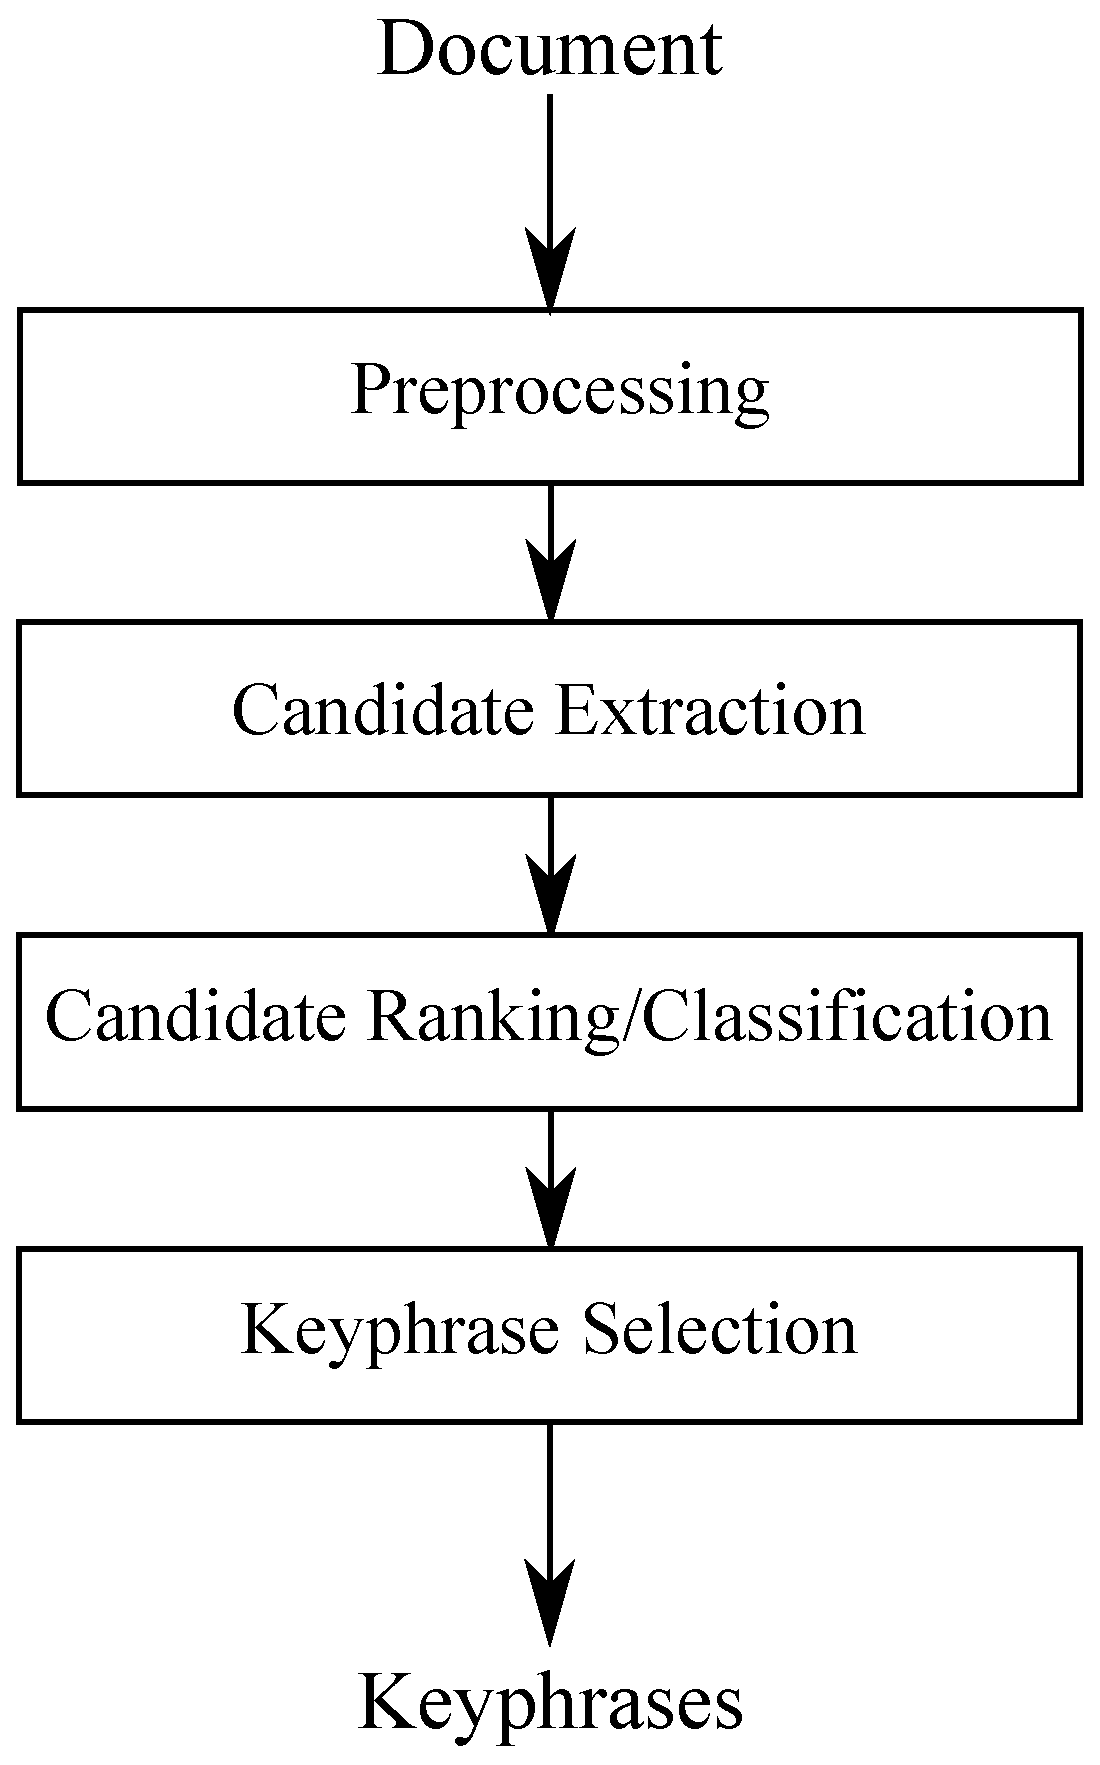
\includegraphics[width=0.3\textwidth]{include/processing_steps.eps}
    \caption{Processing steps of automatic keyphrase extraction methods.
             \label{fig:processing_steps}}
  \end{figure}

  \subsection{KEA}
  \label{subsec:kea}
  \subsection{TF-IDF}
  \label{subsec:tfidf}
  \subsection{SingleRank}
  \label{subsec:singlerank}
  \subsection{TopicRank}
  \label{subsec:topicrank}

\section{Evaluation Datasets}
\label{sec:evaluation_datasets}
  \todo[inline]{Présentation générale des corpus pour l'extraction de
                termes-clés.}
  \todo[inline]{Présentation des corpus qui seront utilisés}

  \begin{table}[h]
    \centering
    \begin{tabular}{@{~}r@{~~}r@{~~}c@{~~}c@{~}}
      \toprule
      \multicolumn{2}{c}{\multirow{2}{*}[-2pt]{\textbf{Statistics}}} & \multicolumn{2}{c}{\textbf{Corpora}}\\
      \cmidrule{3-4}
      & & DUC & SemEval\\
      \midrule
      \multirow{5}{*}[-2pt]{\begin{sideways}\textbf{Documents}\end{sideways}} & Type & News & Papers\\
      & Documents & 308 & 100\\
      & Tokens/document & & 5176.6\\
      & Keyphrases/document & & 14.7\\
      & Missings keyphrases & & 19.3\%\\
      \addlinespace[\defaultaddspace]
      \multirow{10}{*}[-2pt]{\begin{sideways}\textbf{Keyphrases}\end{sideways}} & Unigrams & & \\
      & Bigrams & & \\
      & Trigrams and more & & \\
      & Containing nouns & & \\
      & Containing adjectives & & \\
      & Containing verbs & & \\
      & Containing adverbs & & \\
      & Containing prepositions & & \\
      & Containing determiners & & \\
      & Containing others & & \\
      \bottomrule
    \end{tabular}
    \caption{Dataset statistics. The missing keyphrase percentage is determined
             based on the stemmed form of the gold standard keyphrases.
             \label{tab:dataset_statistics}}
  \end{table}

  \todo[inline]{Donner les séquences de POS les plus fréquentes dans le gold
                standard.}

\section{Evaluation}
\label{sec:evaluation}
  \todo[inline]{Expliquer les deux évaluations: intrinsèque et extrinsèque.}

  \subsection{Experimental Setting}
  \label{subsec:experimental_setting}

  \subsection{Candidate Extraction}
  \label{subsec:candidate_extraction}
    \todo[inline]{Reprendre les statistiques données en
                  section~\ref{sec:evaluation_datasets}, pour les termes
                  candidats extraits.}
    \todo[inline]{Donner le rappel max et comparer avec la taille des différents
                  ensemble.}
    \todo[inline]{Quels sont les termes candidats communs aux ensembles, le
                  propriétés ?}

  \subsection{Keyphrase Extraction}
  \label{subsec:keyphrase_extraction}
    \todo[inline]{Quelles sont les performances de chaque méthode avec chaque
                  ensemble de termes candidats ?}
    \todo[inline]{Que se passe-t-il lorsque l'on ajoute les termes-clés manquant
                  (mais présents dans le document) aux termes candidats (càd
                  comment les termes candidats non termes-clés de chaque
                  ensemble influent sur les résultats)?}

